\documentclass[a4paper]{book}
\usepackage{a4wide}
\usepackage{makeidx}
\usepackage{fancyhdr}
\usepackage{graphicx}
\usepackage{multicol}
\usepackage{float}
\usepackage{textcomp}
\usepackage{alltt}
\usepackage{times}
\usepackage{ifpdf}
\ifpdf
\usepackage[pdftex,
            pagebackref=true,
            colorlinks=true,
            linkcolor=blue,
            unicode
           ]{hyperref}
\else
\usepackage[ps2pdf,
            pagebackref=true,
            colorlinks=true,
            linkcolor=blue,
            unicode
           ]{hyperref}
\usepackage{pspicture}
\fi
\usepackage[utf8]{inputenc}
\usepackage{doxygen}
\makeindex
\setcounter{tocdepth}{3}
\renewcommand{\footrulewidth}{0.4pt}
\begin{document}
\begin{titlepage}
\vspace*{7cm}
\begin{center}
{\Large Generator Doc \\[1ex]\large 0 }\\
\vspace*{1cm}
{\large Generated by Doxygen 1.5.8}\\
\vspace*{0.5cm}
{\small Tue May 5 15:53:32 2009}\\
\end{center}
\end{titlepage}
\clearemptydoublepage
\pagenumbering{roman}
\tableofcontents
\clearemptydoublepage
\pagenumbering{arabic}
\chapter{Class Index}
\section{Class Hierarchy}
This inheritance list is sorted roughly, but not completely, alphabetically:\begin{CompactList}
\item \contentsline{section}{Equipement}{\pageref{class_equipement}}{}
\begin{CompactList}
\item \contentsline{section}{Pc}{\pageref{class_pc}}{}
\end{CompactList}
\item \contentsline{section}{Generator}{\pageref{class_generator}}{}
\end{CompactList}

\chapter{Class Index}
\section{Class List}
Here are the classes, structs, unions and interfaces with brief descriptions:\begin{CompactList}
\item\contentsline{section}{\hyperlink{class_equipement}{Equipement} (Abstract \hyperlink{class_equipement}{Equipement} Base Class )}{\pageref{class_equipement}}{}
\item\contentsline{section}{\hyperlink{class_generator}{Generator} (The main class of the \hyperlink{class_generator}{Generator} )}{\pageref{class_generator}}{}
\item\contentsline{section}{\hyperlink{class_pc}{Pc} (Subclasse from \hyperlink{class_equipement}{Equipement} )}{\pageref{class_pc}}{}
\end{CompactList}

\chapter{File Index}
\section{File List}
Here is a list of all documented files with brief descriptions:\begin{CompactList}
\item\contentsline{section}{/home/elz/workspace/ns-3-generator/\hyperlink{_equipement_8cpp}{Equipement.cpp} (Abstract \hyperlink{class_equipement}{Equipement} Base Class )}{\pageref{_equipement_8cpp}}{}
\item\contentsline{section}{/home/elz/workspace/ns-3-generator/\hyperlink{_equipement_8h}{Equipement.h} (Abstract \hyperlink{class_equipement}{Equipement} Base Class )}{\pageref{_equipement_8h}}{}
\item\contentsline{section}{/home/elz/workspace/ns-3-generator/\hyperlink{_generator_8cpp}{Generator.cpp} (The main class of the \hyperlink{class_generator}{Generator} )}{\pageref{_generator_8cpp}}{}
\item\contentsline{section}{/home/elz/workspace/ns-3-generator/\hyperlink{_generator_8h}{Generator.h} (The main class of the \hyperlink{class_generator}{Generator} )}{\pageref{_generator_8h}}{}
\item\contentsline{section}{/home/elz/workspace/ns-3-generator/\hyperlink{_pc_8cpp}{Pc.cpp} (Subclasse from \hyperlink{class_equipement}{Equipement} )}{\pageref{_pc_8cpp}}{}
\item\contentsline{section}{/home/elz/workspace/ns-3-generator/\hyperlink{_pc_8h}{Pc.h} (Subclasse from \hyperlink{class_equipement}{Equipement} )}{\pageref{_pc_8h}}{}
\end{CompactList}

\chapter{Class Documentation}
\hypertarget{class_equipement}{
\section{Equipement Class Reference}
\label{class_equipement}\index{Equipement@{Equipement}}
}
Abstract \hyperlink{class_equipement}{Equipement} Base Class.  


{\tt \#include $<$Equipement.h$>$}

Inheritance diagram for Equipement::\begin{figure}[H]
\begin{center}
\leavevmode
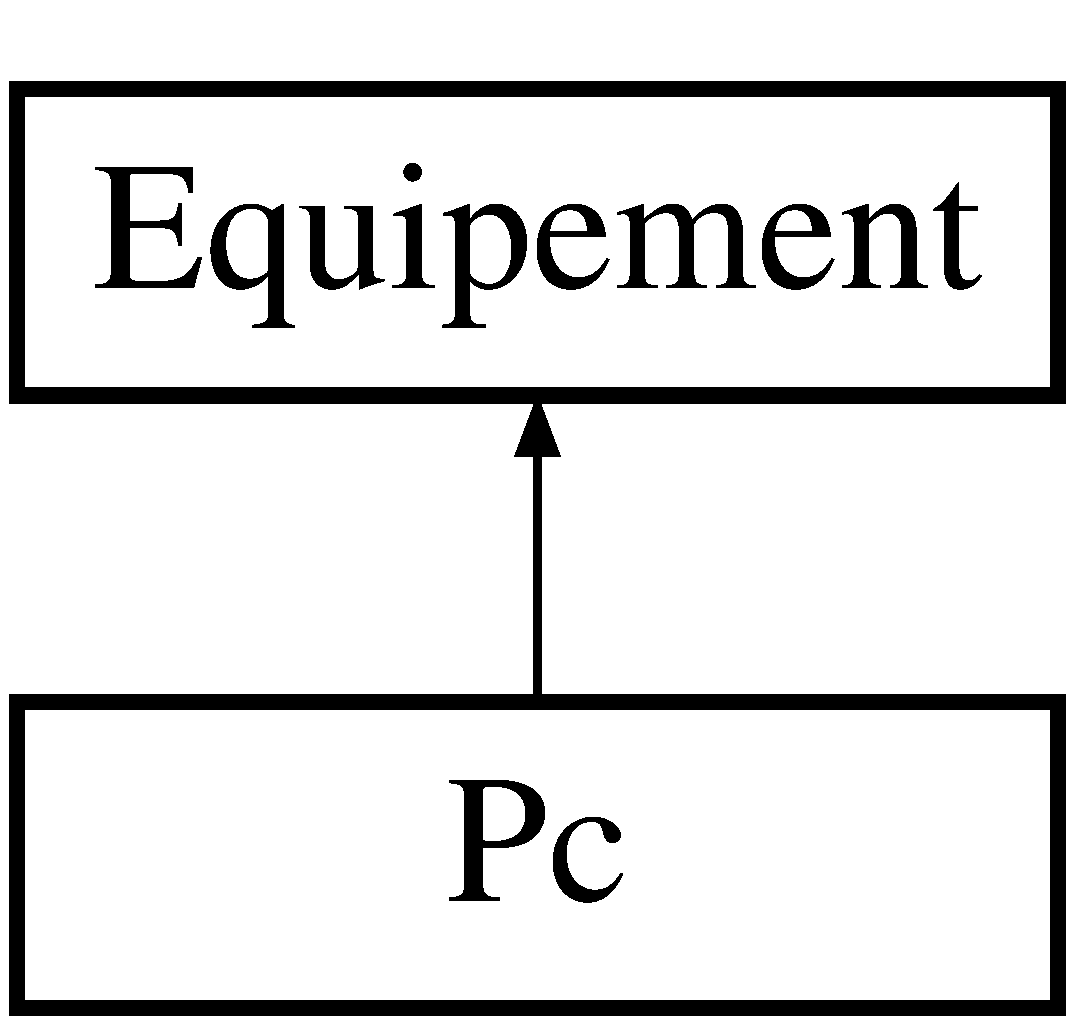
\includegraphics[height=2cm]{class_equipement}
\end{center}
\end{figure}
\subsection*{Public Member Functions}
\begin{CompactItemize}
\item 
\hyperlink{class_equipement_9057a4777d006cbac4c72d09a8d09407}{Equipement} ()
\begin{CompactList}\small\item\em Constructor which set default value. \item\end{CompactList}\item 
virtual \hyperlink{class_equipement_e7751a52f2665d9e4b3e2cd6929bd986}{$\sim$Equipement} ()
\begin{CompactList}\small\item\em Destructor from the class \hyperlink{class_equipement}{Equipement}. \item\end{CompactList}\item 
virtual std::string \hyperlink{class_equipement_136cc8d242b48a665691f8edafa48210}{GenerateHeader} ()=0
\begin{CompactList}\small\item\em Function wich return the c++ header code from node. \item\end{CompactList}\item 
virtual std::string \hyperlink{class_equipement_e03cafed5e059dfe332643719c8d8dd4}{GenerateNode} ()=0
\begin{CompactList}\small\item\em Function wich return the c++ code from node. \item\end{CompactList}\item 
virtual std::string \hyperlink{class_equipement_98eda1e24e07c343712dcd35eba6bd18}{GenerateIpStack} ()=0
\begin{CompactList}\small\item\em Function wich return the c++ code from IpStack. \item\end{CompactList}\item 
virtual std::string \hyperlink{class_equipement_74f771f93374710e8aa42ae17e6b54b4}{GenerateIpAssign} ()=0
\begin{CompactList}\small\item\em Function wich return the c++ code from the ip asssign part. \item\end{CompactList}\item 
virtual void \hyperlink{class_equipement_9068d14ff2c67d06be75a21ebc9fbcd7}{setHeader} (std::string \_\-header)=0
\begin{CompactList}\small\item\em Procedure used to the the c++ header code. \item\end{CompactList}\item 
void \hyperlink{class_equipement_a3d502e4f5b4292e87ff33ca15801897}{setNodeName} (std::string \_\-nodeName)
\begin{CompactList}\small\item\em Procedure to set the node name. \item\end{CompactList}\item 
void \hyperlink{class_equipement_ff68b70ae1942fca75462d78194cd443}{setIpv4Address} (std::string \_\-ip, std::string \_\-mask)
\begin{CompactList}\small\item\em Procedure to set the ip and mask. \item\end{CompactList}\item 
void \hyperlink{class_equipement_cea2da7dead8d0b74c90933c422211c4}{setIpInterfaceName} (std::string \_\-ipInterfaceName)
\begin{CompactList}\small\item\em Procedure to set the Ip interface name. \item\end{CompactList}\item 
void \hyperlink{class_equipement_70bc8e8f1b9527a9c54f4ac6bd93a2c7}{setPosition} (int \_\-x, int \_\-y)
\begin{CompactList}\small\item\em Procedure to set the graphical position of the equipement. \item\end{CompactList}\item 
std::string \hyperlink{class_equipement_4ab70e59e11de8b7f8af99d06409b032}{getNodeName} ()
\begin{CompactList}\small\item\em Function wich return the node name. \item\end{CompactList}\item 
std::string \hyperlink{class_equipement_a603e0547ea7c1b7f10757226100e1cc}{getIpInterfaceName} ()
\begin{CompactList}\small\item\em Function wich return the name of the Ip interface. \item\end{CompactList}\item 
std::string \hyperlink{class_equipement_c4aa745380e69d02a91f1e601430a545}{getHeader} ()
\begin{CompactList}\small\item\em Function wich return the c++ header code. \item\end{CompactList}\item 
std::string \hyperlink{class_equipement_4a0b3805228532e39dcb5f83bb2d6eac}{getIp} ()
\begin{CompactList}\small\item\em Function wich return the ip address. \item\end{CompactList}\item 
std::string \hyperlink{class_equipement_fd9a9ce18e78c3540a0cb6d633def3d3}{getMask} ()
\begin{CompactList}\small\item\em Function wich return a string with the mask. \item\end{CompactList}\item 
std::string \hyperlink{class_equipement_a5f9ea9a69609f65b8c64cda70446b02}{getX} ()
\begin{CompactList}\small\item\em Function which return the x position. \item\end{CompactList}\item 
std::string \hyperlink{class_equipement_a3b627e52bd5bfddadd665ffbf88cbd4}{getY} ()
\begin{CompactList}\small\item\em Function which return the y position. \item\end{CompactList}\item 
std::string \hyperlink{class_equipement_e6b65817f2f2d1f93669475530d849ca}{toString} (int nbr)
\begin{CompactList}\small\item\em Function wich convert int to string. \item\end{CompactList}\item 
std::string \hyperlink{class_equipement_6074ba51d63aaeebe8293a9ba9fde31f}{getIndice} ()
\begin{CompactList}\small\item\em Function wich return the node number. \item\end{CompactList}\end{CompactItemize}
\subsection*{Protected Attributes}
\begin{CompactItemize}
\item 
std::string \hyperlink{class_equipement_d5124abeb4730c781cf45e7d538ebbc2}{indice}
\begin{CompactList}\small\item\em attribute which represent the node number. \item\end{CompactList}\item 
std::string \hyperlink{class_equipement_c83d966d9331f8b92ffa09b5eaf05816}{nodeName}
\begin{CompactList}\small\item\em attribute which represent the node name. \item\end{CompactList}\item 
std::string \hyperlink{class_equipement_0b1a1b3183ff2e26d5e86adcaa1a151d}{ip}
\begin{CompactList}\small\item\em attribute which represent the ip. \item\end{CompactList}\item 
std::string \hyperlink{class_equipement_bc9e4c10eacad003427f4812890c7d52}{mask}
\begin{CompactList}\small\item\em attribute which represent the mask. \item\end{CompactList}\item 
std::string \hyperlink{class_equipement_3e3703936280f99d55619e7b86810f3b}{ipInterfaceName}
\begin{CompactList}\small\item\em attribute which represent the ip interface name. \item\end{CompactList}\item 
std::string \hyperlink{class_equipement_1c7ae76643400f1402231514c2a21ae2}{header}
\begin{CompactList}\small\item\em attribute which represent the header. \item\end{CompactList}\item 
int \hyperlink{class_equipement_45ae2acbe57b1a47e7e9eeed67738109}{x}
\begin{CompactList}\small\item\em attribute which represent the x position of the object. \item\end{CompactList}\item 
int \hyperlink{class_equipement_de92f12b5da5dde6f2b43921789cf676}{y}
\begin{CompactList}\small\item\em attribute which represent the y position of the object. \item\end{CompactList}\end{CompactItemize}


\subsection{Detailed Description}
Abstract \hyperlink{class_equipement}{Equipement} Base Class. 

This class is the main class of the differents equipement you can choose to use. It contain the \hyperlink{class_pc}{Pc}, Hub, Switch, Router, Tap, Wifi Ap, Wifi Station. 

\subsection{Constructor \& Destructor Documentation}
\hypertarget{class_equipement_9057a4777d006cbac4c72d09a8d09407}{
\index{Equipement@{Equipement}!Equipement@{Equipement}}
\index{Equipement@{Equipement}!Equipement@{Equipement}}
\subsubsection[{Equipement}]{\setlength{\rightskip}{0pt plus 5cm}Equipement::Equipement ()}}
\label{class_equipement_9057a4777d006cbac4c72d09a8d09407}


Constructor which set default value. 

The constructor set the default common value at all subclasses. \hypertarget{class_equipement_e7751a52f2665d9e4b3e2cd6929bd986}{
\index{Equipement@{Equipement}!$\sim$Equipement@{$\sim$Equipement}}
\index{$\sim$Equipement@{$\sim$Equipement}!Equipement@{Equipement}}
\subsubsection[{$\sim$Equipement}]{\setlength{\rightskip}{0pt plus 5cm}Equipement::$\sim$Equipement ()\hspace{0.3cm}{\tt  \mbox{[}virtual\mbox{]}}}}
\label{class_equipement_e7751a52f2665d9e4b3e2cd6929bd986}


Destructor from the class \hyperlink{class_equipement}{Equipement}. 

Destructor from the class 

\subsection{Member Function Documentation}
\hypertarget{class_equipement_136cc8d242b48a665691f8edafa48210}{
\index{Equipement@{Equipement}!GenerateHeader@{GenerateHeader}}
\index{GenerateHeader@{GenerateHeader}!Equipement@{Equipement}}
\subsubsection[{GenerateHeader}]{\setlength{\rightskip}{0pt plus 5cm}virtual std::string Equipement::GenerateHeader ()\hspace{0.3cm}{\tt  \mbox{[}pure virtual\mbox{]}}}}
\label{class_equipement_136cc8d242b48a665691f8edafa48210}


Function wich return the c++ header code from node. 

This function return a string which contain the header lines from the specified object. This function have to be rewritten in all subclasses.

\begin{Desc}
\item[Returns:]header. \end{Desc}


Implemented in \hyperlink{class_pc_0b152acc530cc73f502f046e19f9344f}{Pc}.\hypertarget{class_equipement_74f771f93374710e8aa42ae17e6b54b4}{
\index{Equipement@{Equipement}!GenerateIpAssign@{GenerateIpAssign}}
\index{GenerateIpAssign@{GenerateIpAssign}!Equipement@{Equipement}}
\subsubsection[{GenerateIpAssign}]{\setlength{\rightskip}{0pt plus 5cm}virtual std::string Equipement::GenerateIpAssign ()\hspace{0.3cm}{\tt  \mbox{[}pure virtual\mbox{]}}}}
\label{class_equipement_74f771f93374710e8aa42ae17e6b54b4}


Function wich return the c++ code from the ip asssign part. 

This function return a string wich contain the c++ code from the Ipv4 Assign part. It's about ip and mask assign. This function have to be rewritten in all subclasses;

\begin{Desc}
\item[Returns:]IpAssign. \end{Desc}


Implemented in \hyperlink{class_pc_85794eaecd61612d44e1c68746e1c156}{Pc}.\hypertarget{class_equipement_98eda1e24e07c343712dcd35eba6bd18}{
\index{Equipement@{Equipement}!GenerateIpStack@{GenerateIpStack}}
\index{GenerateIpStack@{GenerateIpStack}!Equipement@{Equipement}}
\subsubsection[{GenerateIpStack}]{\setlength{\rightskip}{0pt plus 5cm}virtual std::string Equipement::GenerateIpStack ()\hspace{0.3cm}{\tt  \mbox{[}pure virtual\mbox{]}}}}
\label{class_equipement_98eda1e24e07c343712dcd35eba6bd18}


Function wich return the c++ code from IpStack. 

This function return a string which contain the c++ code from the Ipv4 stack declaration and instanciation. This function have to be rewritten in all subclasses.

\begin{Desc}
\item[Returns:]ipStack. \end{Desc}


Implemented in \hyperlink{class_pc_6b81e7a8e167ed51f92ce55c0447fefe}{Pc}.\hypertarget{class_equipement_e03cafed5e059dfe332643719c8d8dd4}{
\index{Equipement@{Equipement}!GenerateNode@{GenerateNode}}
\index{GenerateNode@{GenerateNode}!Equipement@{Equipement}}
\subsubsection[{GenerateNode}]{\setlength{\rightskip}{0pt plus 5cm}virtual std::string Equipement::GenerateNode ()\hspace{0.3cm}{\tt  \mbox{[}pure virtual\mbox{]}}}}
\label{class_equipement_e03cafed5e059dfe332643719c8d8dd4}


Function wich return the c++ code from node. 

This function return a string which contain the declaration and instanciation of the node. This function have to be rewritten in all subclasses.

\begin{Desc}
\item[Returns:]node. \end{Desc}


Implemented in \hyperlink{class_pc_36ace04642cd481b39d312b51c37c114}{Pc}.\hypertarget{class_equipement_c4aa745380e69d02a91f1e601430a545}{
\index{Equipement@{Equipement}!getHeader@{getHeader}}
\index{getHeader@{getHeader}!Equipement@{Equipement}}
\subsubsection[{getHeader}]{\setlength{\rightskip}{0pt plus 5cm}std::string Equipement::getHeader ()}}
\label{class_equipement_c4aa745380e69d02a91f1e601430a545}


Function wich return the c++ header code. 

Function which return the c++ code from the equipement

\begin{Desc}
\item[Returns:]header c++ code. \end{Desc}
\hypertarget{class_equipement_6074ba51d63aaeebe8293a9ba9fde31f}{
\index{Equipement@{Equipement}!getIndice@{getIndice}}
\index{getIndice@{getIndice}!Equipement@{Equipement}}
\subsubsection[{getIndice}]{\setlength{\rightskip}{0pt plus 5cm}std::string Equipement::getIndice ()}}
\label{class_equipement_6074ba51d63aaeebe8293a9ba9fde31f}


Function wich return the node number. 

Function wich return a string with the node number.

\begin{Desc}
\item[Returns:]node number in type string. \end{Desc}
\hypertarget{class_equipement_4a0b3805228532e39dcb5f83bb2d6eac}{
\index{Equipement@{Equipement}!getIp@{getIp}}
\index{getIp@{getIp}!Equipement@{Equipement}}
\subsubsection[{getIp}]{\setlength{\rightskip}{0pt plus 5cm}std::string Equipement::getIp ()}}
\label{class_equipement_4a0b3805228532e39dcb5f83bb2d6eac}


Function wich return the ip address. 

Function wich return a string with the ip address.

\begin{Desc}
\item[Returns:]ip. \end{Desc}
\hypertarget{class_equipement_a603e0547ea7c1b7f10757226100e1cc}{
\index{Equipement@{Equipement}!getIpInterfaceName@{getIpInterfaceName}}
\index{getIpInterfaceName@{getIpInterfaceName}!Equipement@{Equipement}}
\subsubsection[{getIpInterfaceName}]{\setlength{\rightskip}{0pt plus 5cm}std::string Equipement::getIpInterfaceName ()}}
\label{class_equipement_a603e0547ea7c1b7f10757226100e1cc}


Function wich return the name of the Ip interface. 

Function wich return the ip interface name of the equipement.

\begin{Desc}
\item[Returns:]ip interface name. \end{Desc}
\hypertarget{class_equipement_fd9a9ce18e78c3540a0cb6d633def3d3}{
\index{Equipement@{Equipement}!getMask@{getMask}}
\index{getMask@{getMask}!Equipement@{Equipement}}
\subsubsection[{getMask}]{\setlength{\rightskip}{0pt plus 5cm}std::string Equipement::getMask ()}}
\label{class_equipement_fd9a9ce18e78c3540a0cb6d633def3d3}


Function wich return a string with the mask. 

Function wich return a string with the mask.

\begin{Desc}
\item[Returns:]mask. \end{Desc}
\hypertarget{class_equipement_4ab70e59e11de8b7f8af99d06409b032}{
\index{Equipement@{Equipement}!getNodeName@{getNodeName}}
\index{getNodeName@{getNodeName}!Equipement@{Equipement}}
\subsubsection[{getNodeName}]{\setlength{\rightskip}{0pt plus 5cm}std::string Equipement::getNodeName ()}}
\label{class_equipement_4ab70e59e11de8b7f8af99d06409b032}


Function wich return the node name. 

function used to get the node name of the equipement.

\begin{Desc}
\item[Returns:]node name. \end{Desc}
\hypertarget{class_equipement_a5f9ea9a69609f65b8c64cda70446b02}{
\index{Equipement@{Equipement}!getX@{getX}}
\index{getX@{getX}!Equipement@{Equipement}}
\subsubsection[{getX}]{\setlength{\rightskip}{0pt plus 5cm}std::string Equipement::getX ()}}
\label{class_equipement_a5f9ea9a69609f65b8c64cda70446b02}


Function which return the x position. 

Function wich return the graphical x position of the object.

\begin{Desc}
\item[Returns:]x position. \end{Desc}
\hypertarget{class_equipement_a3b627e52bd5bfddadd665ffbf88cbd4}{
\index{Equipement@{Equipement}!getY@{getY}}
\index{getY@{getY}!Equipement@{Equipement}}
\subsubsection[{getY}]{\setlength{\rightskip}{0pt plus 5cm}std::string Equipement::getY ()}}
\label{class_equipement_a3b627e52bd5bfddadd665ffbf88cbd4}


Function which return the y position. 

Function wich return the graphical y position of the object.

\begin{Desc}
\item[Returns:]y position. \end{Desc}
\hypertarget{class_equipement_9068d14ff2c67d06be75a21ebc9fbcd7}{
\index{Equipement@{Equipement}!setHeader@{setHeader}}
\index{setHeader@{setHeader}!Equipement@{Equipement}}
\subsubsection[{setHeader}]{\setlength{\rightskip}{0pt plus 5cm}virtual void Equipement::setHeader (std::string {\em \_\-header})\hspace{0.3cm}{\tt  \mbox{[}pure virtual\mbox{]}}}}
\label{class_equipement_9068d14ff2c67d06be75a21ebc9fbcd7}


Procedure used to the the c++ header code. 

This procedure is used to set the header c++ code as a string. It's used to generate the code. This procedure have to be rewritted un all subclasses.

\begin{Desc}
\item[Parameters:]
\begin{description}
\item[{\em \_\-header}]the header which have to be set. \end{description}
\end{Desc}


Implemented in \hyperlink{class_pc_8049628cd139b39cbae2327e70ca0eb7}{Pc}.\hypertarget{class_equipement_cea2da7dead8d0b74c90933c422211c4}{
\index{Equipement@{Equipement}!setIpInterfaceName@{setIpInterfaceName}}
\index{setIpInterfaceName@{setIpInterfaceName}!Equipement@{Equipement}}
\subsubsection[{setIpInterfaceName}]{\setlength{\rightskip}{0pt plus 5cm}void Equipement::setIpInterfaceName (std::string {\em \_\-ipInterfaceName})}}
\label{class_equipement_cea2da7dead8d0b74c90933c422211c4}


Procedure to set the Ip interface name. 

This procedure is used to the the ipInterfaceName. Sometimes this var is used in application like an UdpEcho.

\begin{Desc}
\item[Parameters:]
\begin{description}
\item[{\em \_\-ipInterfaceName}]\end{description}
\end{Desc}
\hypertarget{class_equipement_ff68b70ae1942fca75462d78194cd443}{
\index{Equipement@{Equipement}!setIpv4Address@{setIpv4Address}}
\index{setIpv4Address@{setIpv4Address}!Equipement@{Equipement}}
\subsubsection[{setIpv4Address}]{\setlength{\rightskip}{0pt plus 5cm}void Equipement::setIpv4Address (std::string {\em \_\-ip}, \/  std::string {\em \_\-mask})}}
\label{class_equipement_ff68b70ae1942fca75462d78194cd443}


Procedure to set the ip and mask. 

The ip have to be inserted as an ipv4 address. Example :10.0.0.1 Mask example : 255.255.255.0

\begin{Desc}
\item[Parameters:]
\begin{description}
\item[{\em \_\-ip}]the ip. \item[{\em \_\-mask}]the mask. \end{description}
\end{Desc}
\hypertarget{class_equipement_a3d502e4f5b4292e87ff33ca15801897}{
\index{Equipement@{Equipement}!setNodeName@{setNodeName}}
\index{setNodeName@{setNodeName}!Equipement@{Equipement}}
\subsubsection[{setNodeName}]{\setlength{\rightskip}{0pt plus 5cm}void Equipement::setNodeName (std::string {\em \_\-nodeName})}}
\label{class_equipement_a3d502e4f5b4292e87ff33ca15801897}


Procedure to set the node name. 

The node name is use to declare and instace the node in the c++ generated code.

\begin{Desc}
\item[Parameters:]
\begin{description}
\item[{\em \_\-nodeName}]the string which containe the node name. \end{description}
\end{Desc}
\hypertarget{class_equipement_70bc8e8f1b9527a9c54f4ac6bd93a2c7}{
\index{Equipement@{Equipement}!setPosition@{setPosition}}
\index{setPosition@{setPosition}!Equipement@{Equipement}}
\subsubsection[{setPosition}]{\setlength{\rightskip}{0pt plus 5cm}void Equipement::setPosition (int {\em \_\-x}, \/  int {\em \_\-y})}}
\label{class_equipement_70bc8e8f1b9527a9c54f4ac6bd93a2c7}


Procedure to set the graphical position of the equipement. 

This procedure is used to change the position of an equipement. Like after a drag n drop.

\begin{Desc}
\item[Parameters:]
\begin{description}
\item[{\em \_\-x}]the x position. \item[{\em \_\-y}]the y position. \end{description}
\end{Desc}
\hypertarget{class_equipement_e6b65817f2f2d1f93669475530d849ca}{
\index{Equipement@{Equipement}!toString@{toString}}
\index{toString@{toString}!Equipement@{Equipement}}
\subsubsection[{toString}]{\setlength{\rightskip}{0pt plus 5cm}std::string Equipement::toString (int {\em nbr})}}
\label{class_equipement_e6b65817f2f2d1f93669475530d849ca}


Function wich convert int to string. 

Function wich convert in to string.

\begin{Desc}
\item[Parameters:]
\begin{description}
\item[{\em nbr}]the number to convert. \end{description}
\end{Desc}
\begin{Desc}
\item[Returns:]nbr in type string. \end{Desc}


\subsection{Member Data Documentation}
\hypertarget{class_equipement_1c7ae76643400f1402231514c2a21ae2}{
\index{Equipement@{Equipement}!header@{header}}
\index{header@{header}!Equipement@{Equipement}}
\subsubsection[{header}]{\setlength{\rightskip}{0pt plus 5cm}std::string {\bf Equipement::header}\hspace{0.3cm}{\tt  \mbox{[}protected\mbox{]}}}}
\label{class_equipement_1c7ae76643400f1402231514c2a21ae2}


attribute which represent the header. 

This attribute reprensent the differents files to be included for the node. \hypertarget{class_equipement_d5124abeb4730c781cf45e7d538ebbc2}{
\index{Equipement@{Equipement}!indice@{indice}}
\index{indice@{indice}!Equipement@{Equipement}}
\subsubsection[{indice}]{\setlength{\rightskip}{0pt plus 5cm}std::string {\bf Equipement::indice}\hspace{0.3cm}{\tt  \mbox{[}protected\mbox{]}}}}
\label{class_equipement_d5124abeb4730c781cf45e7d538ebbc2}


attribute which represent the node number. 

This is an attribute which represent the number of the object creation. \hypertarget{class_equipement_0b1a1b3183ff2e26d5e86adcaa1a151d}{
\index{Equipement@{Equipement}!ip@{ip}}
\index{ip@{ip}!Equipement@{Equipement}}
\subsubsection[{ip}]{\setlength{\rightskip}{0pt plus 5cm}std::string {\bf Equipement::ip}\hspace{0.3cm}{\tt  \mbox{[}protected\mbox{]}}}}
\label{class_equipement_0b1a1b3183ff2e26d5e86adcaa1a151d}


attribute which represent the ip. 

The ip attributed to the node. \hypertarget{class_equipement_3e3703936280f99d55619e7b86810f3b}{
\index{Equipement@{Equipement}!ipInterfaceName@{ipInterfaceName}}
\index{ipInterfaceName@{ipInterfaceName}!Equipement@{Equipement}}
\subsubsection[{ipInterfaceName}]{\setlength{\rightskip}{0pt plus 5cm}std::string {\bf Equipement::ipInterfaceName}\hspace{0.3cm}{\tt  \mbox{[}protected\mbox{]}}}}
\label{class_equipement_3e3703936280f99d55619e7b86810f3b}


attribute which represent the ip interface name. 

The ip interface name is used to generate the code for the applications like an udp\_\-echo. \hypertarget{class_equipement_bc9e4c10eacad003427f4812890c7d52}{
\index{Equipement@{Equipement}!mask@{mask}}
\index{mask@{mask}!Equipement@{Equipement}}
\subsubsection[{mask}]{\setlength{\rightskip}{0pt plus 5cm}std::string {\bf Equipement::mask}\hspace{0.3cm}{\tt  \mbox{[}protected\mbox{]}}}}
\label{class_equipement_bc9e4c10eacad003427f4812890c7d52}


attribute which represent the mask. 

The mask attributed to the node network. \hypertarget{class_equipement_c83d966d9331f8b92ffa09b5eaf05816}{
\index{Equipement@{Equipement}!nodeName@{nodeName}}
\index{nodeName@{nodeName}!Equipement@{Equipement}}
\subsubsection[{nodeName}]{\setlength{\rightskip}{0pt plus 5cm}std::string {\bf Equipement::nodeName}\hspace{0.3cm}{\tt  \mbox{[}protected\mbox{]}}}}
\label{class_equipement_c83d966d9331f8b92ffa09b5eaf05816}


attribute which represent the node name. 

The node name. \hypertarget{class_equipement_45ae2acbe57b1a47e7e9eeed67738109}{
\index{Equipement@{Equipement}!x@{x}}
\index{x@{x}!Equipement@{Equipement}}
\subsubsection[{x}]{\setlength{\rightskip}{0pt plus 5cm}int {\bf Equipement::x}\hspace{0.3cm}{\tt  \mbox{[}protected\mbox{]}}}}
\label{class_equipement_45ae2acbe57b1a47e7e9eeed67738109}


attribute which represent the x position of the object. 

The x graphical position. \hypertarget{class_equipement_de92f12b5da5dde6f2b43921789cf676}{
\index{Equipement@{Equipement}!y@{y}}
\index{y@{y}!Equipement@{Equipement}}
\subsubsection[{y}]{\setlength{\rightskip}{0pt plus 5cm}int {\bf Equipement::y}\hspace{0.3cm}{\tt  \mbox{[}protected\mbox{]}}}}
\label{class_equipement_de92f12b5da5dde6f2b43921789cf676}


attribute which represent the y position of the object. 

The y graphical position. 

The documentation for this class was generated from the following files:\begin{CompactItemize}
\item 
/home/elz/workspace/ns-3-generator/\hyperlink{_equipement_8h}{Equipement.h}\item 
/home/elz/workspace/ns-3-generator/\hyperlink{_equipement_8cpp}{Equipement.cpp}\end{CompactItemize}

\hypertarget{class_generator}{
\section{Generator Class Reference}
\label{class_generator}\index{Generator@{Generator}}
}
The main class of the \hyperlink{class_generator}{Generator}.  


{\tt \#include $<$Generator.h$>$}

\subsection*{Public Member Functions}
\begin{CompactItemize}
\item 
\hyperlink{class_generator_aaf1e5f3a47ede3ef8a96a301ee04a10}{Generator} ()
\begin{CompactList}\small\item\em the generator of the class \hyperlink{class_generator}{Generator}. \item\end{CompactList}\item 
void \hyperlink{class_generator_caee4fe4990cee0447f0cb27ef413c9b}{GenerateCode} ()
\begin{CompactList}\small\item\em Procedure wich are the main code generator. \item\end{CompactList}\end{CompactItemize}
\subsection*{Static Public Member Functions}
\begin{CompactItemize}
\item 
static void \hyperlink{class_generator_a8745946602d6e64e5b131d682737e77}{AddEquipement} (std::string type)
\begin{CompactList}\small\item\em Procedure used to add an equipement. \item\end{CompactList}\item 
static int \hyperlink{class_generator_714d17823705b75edfbb9bbe37d35c7a}{getIndiceEquipement} ()
\begin{CompactList}\small\item\em Function wich return the number of equipement created. \item\end{CompactList}\item 
static void \hyperlink{class_generator_bd0054d3e88aaeda093ac882861d6410}{AddApplication} (std::string type)
\begin{CompactList}\small\item\em list of application created instace. \item\end{CompactList}\item 
static int \hyperlink{class_generator_32a1fcc314ade484d84669ac7e510e68}{getIndiceApplication} ()
\begin{CompactList}\small\item\em Function wich return the number of application created. \item\end{CompactList}\item 
static void \hyperlink{class_generator_3fe9d83270bd9d22b9307d3b0a26ea39}{AddLink} (std::string type)
\begin{CompactList}\small\item\em list of link created instace. \item\end{CompactList}\item 
static int \hyperlink{class_generator_05e1b6e209fb7730960de318fccaa86a}{getIndiceLink} ()
\begin{CompactList}\small\item\em Function wich return the number of link created. \item\end{CompactList}\end{CompactItemize}
\subsection*{Static Public Attributes}
\begin{CompactItemize}
\item 
static std::vector$<$ \hyperlink{class_equipement}{Equipement} $\ast$ $>$ \hyperlink{class_generator_96d452a5ef951497a37baf86e35b50f6}{listEquipement}
\begin{CompactList}\small\item\em list of equipement created instace. \item\end{CompactList}\end{CompactItemize}


\subsection{Detailed Description}
The main class of the \hyperlink{class_generator}{Generator}. 

This class is the main class from the generation of simulation. It containt the main method to generate the code for the simulation. 

\subsection{Constructor \& Destructor Documentation}
\hypertarget{class_generator_aaf1e5f3a47ede3ef8a96a301ee04a10}{
\index{Generator@{Generator}!Generator@{Generator}}
\index{Generator@{Generator}!Generator@{Generator}}
\subsubsection[{Generator}]{\setlength{\rightskip}{0pt plus 5cm}Generator::Generator ()}}
\label{class_generator_aaf1e5f3a47ede3ef8a96a301ee04a10}


the generator of the class \hyperlink{class_generator}{Generator}. 

The generator from the class. 

\subsection{Member Function Documentation}
\hypertarget{class_generator_bd0054d3e88aaeda093ac882861d6410}{
\index{Generator@{Generator}!AddApplication@{AddApplication}}
\index{AddApplication@{AddApplication}!Generator@{Generator}}
\subsubsection[{AddApplication}]{\setlength{\rightskip}{0pt plus 5cm}void Generator::AddApplication (std::string {\em type})\hspace{0.3cm}{\tt  \mbox{[}static\mbox{]}}}}
\label{class_generator_bd0054d3e88aaeda093ac882861d6410}


list of application created instace. 

This attribute is the list of the created application of equipement. Procedure used to add an application. This procedure is used to add an application. It add the application to the vector listApplication and increment the number of application.

\begin{Desc}
\item[Parameters:]
\begin{description}
\item[{\em type}]the type of the application. (Ping, Udp\_\-Echo,...) \end{description}
\end{Desc}
\hypertarget{class_generator_a8745946602d6e64e5b131d682737e77}{
\index{Generator@{Generator}!AddEquipement@{AddEquipement}}
\index{AddEquipement@{AddEquipement}!Generator@{Generator}}
\subsubsection[{AddEquipement}]{\setlength{\rightskip}{0pt plus 5cm}void Generator::AddEquipement (std::string {\em type})\hspace{0.3cm}{\tt  \mbox{[}static\mbox{]}}}}
\label{class_generator_a8745946602d6e64e5b131d682737e77}


Procedure used to add an equipement. 

This procedure is used to add an equipement. It add the equipement to the vector listEquipement and increment the number of equipement.

\begin{Desc}
\item[Parameters:]
\begin{description}
\item[{\em type}]the type of the equipement. (\hyperlink{class_pc}{Pc}, Hub, Switch,...) \end{description}
\end{Desc}
\hypertarget{class_generator_3fe9d83270bd9d22b9307d3b0a26ea39}{
\index{Generator@{Generator}!AddLink@{AddLink}}
\index{AddLink@{AddLink}!Generator@{Generator}}
\subsubsection[{AddLink}]{\setlength{\rightskip}{0pt plus 5cm}void Generator::AddLink (std::string {\em type})\hspace{0.3cm}{\tt  \mbox{[}static\mbox{]}}}}
\label{class_generator_3fe9d83270bd9d22b9307d3b0a26ea39}


list of link created instace. 

This attribute is the list of the created instance of link. Procedure used to add an link. This procedure is used to add an link. It add the link to the vector listLink and increment the number of link.

\begin{Desc}
\item[Parameters:]
\begin{description}
\item[{\em type}]the type of the link. (PointToPoint, Csma,...) \end{description}
\end{Desc}
\hypertarget{class_generator_caee4fe4990cee0447f0cb27ef413c9b}{
\index{Generator@{Generator}!GenerateCode@{GenerateCode}}
\index{GenerateCode@{GenerateCode}!Generator@{Generator}}
\subsubsection[{GenerateCode}]{\setlength{\rightskip}{0pt plus 5cm}void Generator::GenerateCode ()}}
\label{class_generator_caee4fe4990cee0447f0cb27ef413c9b}


Procedure wich are the main code generator. 

This procedure is the main procedure to generate the code from the simulation. It also go to use all the procedure on the bottom like generate all headers, ... \hypertarget{class_generator_32a1fcc314ade484d84669ac7e510e68}{
\index{Generator@{Generator}!getIndiceApplication@{getIndiceApplication}}
\index{getIndiceApplication@{getIndiceApplication}!Generator@{Generator}}
\subsubsection[{getIndiceApplication}]{\setlength{\rightskip}{0pt plus 5cm}int Generator::getIndiceApplication ()\hspace{0.3cm}{\tt  \mbox{[}static\mbox{]}}}}
\label{class_generator_32a1fcc314ade484d84669ac7e510e68}


Function wich return the number of application created. 

This function return the number of application created.

\begin{Desc}
\item[Returns:]number of application \end{Desc}
\hypertarget{class_generator_714d17823705b75edfbb9bbe37d35c7a}{
\index{Generator@{Generator}!getIndiceEquipement@{getIndiceEquipement}}
\index{getIndiceEquipement@{getIndiceEquipement}!Generator@{Generator}}
\subsubsection[{getIndiceEquipement}]{\setlength{\rightskip}{0pt plus 5cm}int Generator::getIndiceEquipement ()\hspace{0.3cm}{\tt  \mbox{[}static\mbox{]}}}}
\label{class_generator_714d17823705b75edfbb9bbe37d35c7a}


Function wich return the number of equipement created. 

This function return the number of equipement created in the application.

\begin{Desc}
\item[Returns:]number of equipement \end{Desc}
\hypertarget{class_generator_05e1b6e209fb7730960de318fccaa86a}{
\index{Generator@{Generator}!getIndiceLink@{getIndiceLink}}
\index{getIndiceLink@{getIndiceLink}!Generator@{Generator}}
\subsubsection[{getIndiceLink}]{\setlength{\rightskip}{0pt plus 5cm}int Generator::getIndiceLink ()\hspace{0.3cm}{\tt  \mbox{[}static\mbox{]}}}}
\label{class_generator_05e1b6e209fb7730960de318fccaa86a}


Function wich return the number of link created. 

This function return the number of link created in the application.

\begin{Desc}
\item[Returns:]number of link \end{Desc}


\subsection{Member Data Documentation}
\hypertarget{class_generator_96d452a5ef951497a37baf86e35b50f6}{
\index{Generator@{Generator}!listEquipement@{listEquipement}}
\index{listEquipement@{listEquipement}!Generator@{Generator}}
\subsubsection[{listEquipement}]{\setlength{\rightskip}{0pt plus 5cm}std::vector$<$ {\bf Equipement} $\ast$ $>$ {\bf Generator::listEquipement}\hspace{0.3cm}{\tt  \mbox{[}static\mbox{]}}}}
\label{class_generator_96d452a5ef951497a37baf86e35b50f6}


list of equipement created instace. 

This attribute is the list of the created instance of equipement. 

The documentation for this class was generated from the following files:\begin{CompactItemize}
\item 
/home/elz/workspace/ns-3-generator/\hyperlink{_generator_8h}{Generator.h}\item 
/home/elz/workspace/ns-3-generator/\hyperlink{_generator_8cpp}{Generator.cpp}\end{CompactItemize}

\hypertarget{class_pc}{
\section{Pc Class Reference}
\label{class_pc}\index{Pc@{Pc}}
}
Subclasse from \hyperlink{class_equipement}{Equipement}.  


{\tt \#include $<$Pc.h$>$}

Inheritance diagram for Pc::\begin{figure}[H]
\begin{center}
\leavevmode
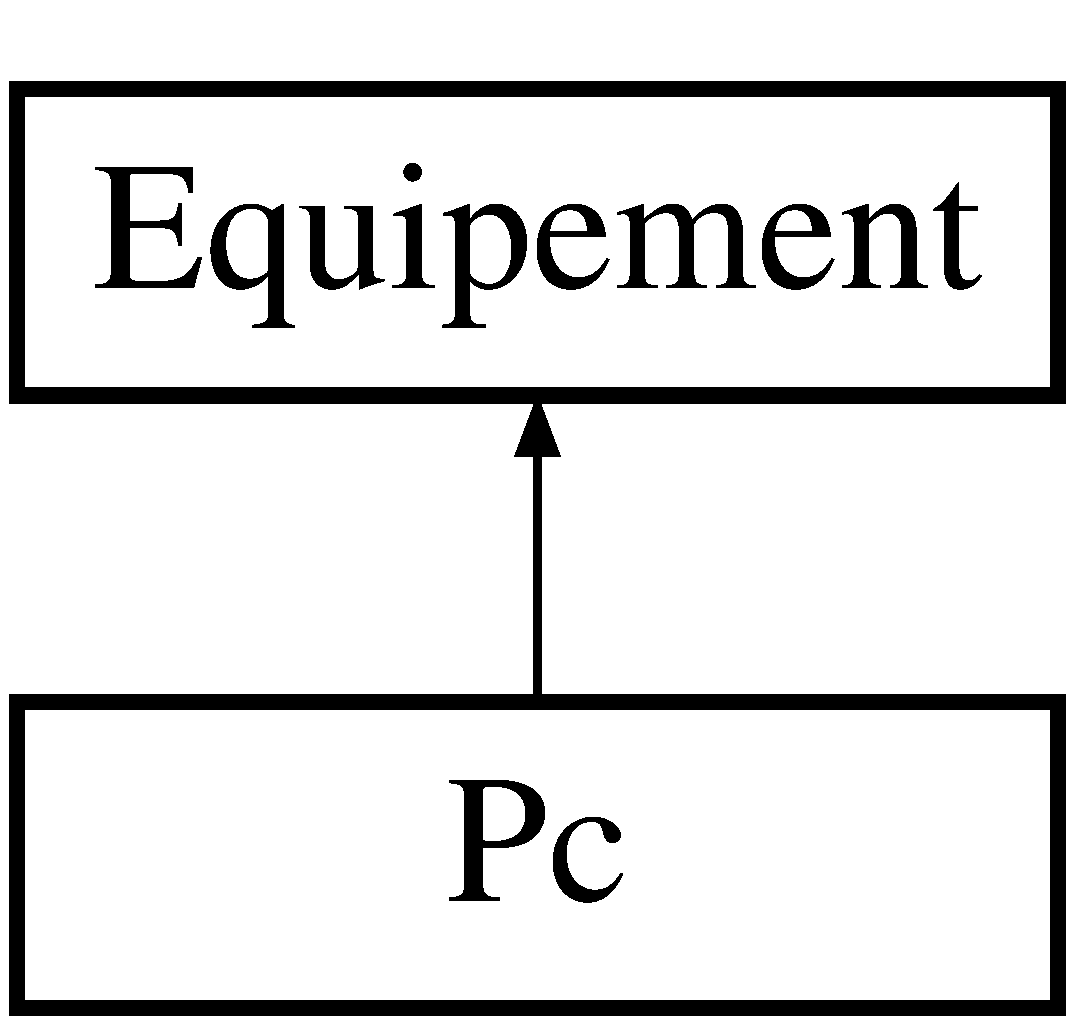
\includegraphics[height=2cm]{class_pc}
\end{center}
\end{figure}
\subsection*{Public Member Functions}
\begin{CompactItemize}
\item 
\hyperlink{class_pc_ef7314496cee3c1bd2c329aac4dc4f21}{Pc} ()
\begin{CompactList}\small\item\em Constructor used for a \hyperlink{class_pc}{Pc}. \item\end{CompactList}\item 
virtual \hyperlink{class_pc_b15cb9b9bfb8a9d9ff964091e1a63cec}{$\sim$Pc} ()
\begin{CompactList}\small\item\em the destructor of the class. \item\end{CompactList}\item 
virtual std::string \hyperlink{class_pc_0b152acc530cc73f502f046e19f9344f}{GenerateHeader} ()
\begin{CompactList}\small\item\em Function witch return the header c++ code. \item\end{CompactList}\item 
virtual std::string \hyperlink{class_pc_36ace04642cd481b39d312b51c37c114}{GenerateNode} ()
\begin{CompactList}\small\item\em Function witch return the node c++ code. \item\end{CompactList}\item 
virtual std::string \hyperlink{class_pc_6b81e7a8e167ed51f92ce55c0447fefe}{GenerateIpStack} ()
\begin{CompactList}\small\item\em Function witch return the ip stack c++ code. \item\end{CompactList}\item 
virtual std::string \hyperlink{class_pc_85794eaecd61612d44e1c68746e1c156}{GenerateIpAssign} ()
\begin{CompactList}\small\item\em Function witch return the ip assign c++ code. \item\end{CompactList}\item 
virtual void \hyperlink{class_pc_8049628cd139b39cbae2327e70ca0eb7}{setHeader} (std::string \_\-header)
\begin{CompactList}\small\item\em Function witch set the header c++ code. \item\end{CompactList}\end{CompactItemize}


\subsection{Detailed Description}
Subclasse from \hyperlink{class_equipement}{Equipement}. 

This class is a subclass from main class \hyperlink{class_equipement}{Equipement}. It reprensent a simple pc. 

\subsection{Constructor \& Destructor Documentation}
\hypertarget{class_pc_ef7314496cee3c1bd2c329aac4dc4f21}{
\index{Pc@{Pc}!Pc@{Pc}}
\index{Pc@{Pc}!Pc@{Pc}}
\subsubsection[{Pc}]{\setlength{\rightskip}{0pt plus 5cm}Pc::Pc ()}}
\label{class_pc_ef7314496cee3c1bd2c329aac4dc4f21}


Constructor used for a \hyperlink{class_pc}{Pc}. 

This is the constructor of the \hyperlink{class_pc}{Pc} class. This object rewrite the virtual method from main class. It also contain the c++ code specific from a \hyperlink{class_pc}{Pc}. \hypertarget{class_pc_b15cb9b9bfb8a9d9ff964091e1a63cec}{
\index{Pc@{Pc}!$\sim$Pc@{$\sim$Pc}}
\index{$\sim$Pc@{$\sim$Pc}!Pc@{Pc}}
\subsubsection[{$\sim$Pc}]{\setlength{\rightskip}{0pt plus 5cm}Pc::$\sim$Pc ()\hspace{0.3cm}{\tt  \mbox{[}virtual\mbox{]}}}}
\label{class_pc_b15cb9b9bfb8a9d9ff964091e1a63cec}


the destructor of the class. 

The class destructor. 

\subsection{Member Function Documentation}
\hypertarget{class_pc_0b152acc530cc73f502f046e19f9344f}{
\index{Pc@{Pc}!GenerateHeader@{GenerateHeader}}
\index{GenerateHeader@{GenerateHeader}!Pc@{Pc}}
\subsubsection[{GenerateHeader}]{\setlength{\rightskip}{0pt plus 5cm}std::string Pc::GenerateHeader ()\hspace{0.3cm}{\tt  \mbox{[}virtual\mbox{]}}}}
\label{class_pc_0b152acc530cc73f502f046e19f9344f}


Function witch return the header c++ code. 

Function wich return a string with the header c++ code from a \hyperlink{class_pc}{Pc}.

\begin{Desc}
\item[Returns:]header. \end{Desc}


Implements \hyperlink{class_equipement_136cc8d242b48a665691f8edafa48210}{Equipement}.\hypertarget{class_pc_85794eaecd61612d44e1c68746e1c156}{
\index{Pc@{Pc}!GenerateIpAssign@{GenerateIpAssign}}
\index{GenerateIpAssign@{GenerateIpAssign}!Pc@{Pc}}
\subsubsection[{GenerateIpAssign}]{\setlength{\rightskip}{0pt plus 5cm}std::string Pc::GenerateIpAssign ()\hspace{0.3cm}{\tt  \mbox{[}virtual\mbox{]}}}}
\label{class_pc_85794eaecd61612d44e1c68746e1c156}


Function witch return the ip assign c++ code. 

Function wich return a string with the ip assign c++ code from a \hyperlink{class_pc}{Pc}.

\begin{Desc}
\item[Returns:]ip assign. \end{Desc}


Implements \hyperlink{class_equipement_74f771f93374710e8aa42ae17e6b54b4}{Equipement}.\hypertarget{class_pc_6b81e7a8e167ed51f92ce55c0447fefe}{
\index{Pc@{Pc}!GenerateIpStack@{GenerateIpStack}}
\index{GenerateIpStack@{GenerateIpStack}!Pc@{Pc}}
\subsubsection[{GenerateIpStack}]{\setlength{\rightskip}{0pt plus 5cm}std::string Pc::GenerateIpStack ()\hspace{0.3cm}{\tt  \mbox{[}virtual\mbox{]}}}}
\label{class_pc_6b81e7a8e167ed51f92ce55c0447fefe}


Function witch return the ip stack c++ code. 

Function wich return a string with the ip stack c++ code from a \hyperlink{class_pc}{Pc}.

\begin{Desc}
\item[Returns:]ip stack. \end{Desc}


Implements \hyperlink{class_equipement_98eda1e24e07c343712dcd35eba6bd18}{Equipement}.\hypertarget{class_pc_36ace04642cd481b39d312b51c37c114}{
\index{Pc@{Pc}!GenerateNode@{GenerateNode}}
\index{GenerateNode@{GenerateNode}!Pc@{Pc}}
\subsubsection[{GenerateNode}]{\setlength{\rightskip}{0pt plus 5cm}std::string Pc::GenerateNode ()\hspace{0.3cm}{\tt  \mbox{[}virtual\mbox{]}}}}
\label{class_pc_36ace04642cd481b39d312b51c37c114}


Function witch return the node c++ code. 

Function wich return a string with the node c++ code from a \hyperlink{class_pc}{Pc}.

\begin{Desc}
\item[Returns:]node. \end{Desc}


Implements \hyperlink{class_equipement_e03cafed5e059dfe332643719c8d8dd4}{Equipement}.\hypertarget{class_pc_8049628cd139b39cbae2327e70ca0eb7}{
\index{Pc@{Pc}!setHeader@{setHeader}}
\index{setHeader@{setHeader}!Pc@{Pc}}
\subsubsection[{setHeader}]{\setlength{\rightskip}{0pt plus 5cm}void Pc::setHeader (std::string {\em \_\-header})\hspace{0.3cm}{\tt  \mbox{[}virtual\mbox{]}}}}
\label{class_pc_8049628cd139b39cbae2327e70ca0eb7}


Function witch set the header c++ code. 

Function wich set the c++ code from the \hyperlink{class_pc}{Pc}.

\begin{Desc}
\item[Parameters:]
\begin{description}
\item[{\em \_\-header}]the new header string. \end{description}
\end{Desc}


Implements \hyperlink{class_equipement_9068d14ff2c67d06be75a21ebc9fbcd7}{Equipement}.

The documentation for this class was generated from the following files:\begin{CompactItemize}
\item 
/home/elz/workspace/ns-3-generator/\hyperlink{_pc_8h}{Pc.h}\item 
/home/elz/workspace/ns-3-generator/\hyperlink{_pc_8cpp}{Pc.cpp}\end{CompactItemize}

\chapter{File Documentation}
\hypertarget{_equipement_8cpp}{
\section{/home/elz/workspace/ns-3-generator/Equipement.cpp File Reference}
\label{_equipement_8cpp}\index{/home/elz/workspace/ns-3-generator/Equipement.cpp@{/home/elz/workspace/ns-3-generator/Equipement.cpp}}
}
Abstract \hyperlink{class_equipement}{Equipement} Base Class.  


{\tt \#include \char`\"{}Equipement.h\char`\"{}}\par
{\tt \#include \char`\"{}Generator.h\char`\"{}}\par
{\tt \#include $<$sstream$>$}\par


\subsection{Detailed Description}
Abstract \hyperlink{class_equipement}{Equipement} Base Class. 

\begin{Desc}
\item[Author:]Pierre Weiss \end{Desc}
\begin{Desc}
\item[Date:]2009 \end{Desc}

\hypertarget{_equipement_8h}{
\section{/home/elz/workspace/ns-3-generator/Equipement.h File Reference}
\label{_equipement_8h}\index{/home/elz/workspace/ns-3-generator/Equipement.h@{/home/elz/workspace/ns-3-generator/Equipement.h}}
}
Abstract \hyperlink{class_equipement}{Equipement} Base Class.  


{\tt \#include $<$iostream$>$}\par
{\tt \#include $<$string$>$}\par
{\tt \#include $<$vector$>$}\par
\subsection*{Classes}
\begin{CompactItemize}
\item 
class \hyperlink{class_equipement}{Equipement}
\begin{CompactList}\small\item\em Abstract \hyperlink{class_equipement}{Equipement} Base Class. \item\end{CompactList}\end{CompactItemize}


\subsection{Detailed Description}
Abstract \hyperlink{class_equipement}{Equipement} Base Class. 

\begin{Desc}
\item[Author:]Pierre Weiss \end{Desc}
\begin{Desc}
\item[Date:]2009 \end{Desc}

\hypertarget{_generator_8cpp}{
\section{/home/elz/workspace/ns-3-generator/Generator.cpp File Reference}
\label{_generator_8cpp}\index{/home/elz/workspace/ns-3-generator/Generator.cpp@{/home/elz/workspace/ns-3-generator/Generator.cpp}}
}
The main class of the \hyperlink{class_generator}{Generator}.  


{\tt \#include \char`\"{}Generator.h\char`\"{}}\par
{\tt \#include \char`\"{}Equipement.h\char`\"{}}\par
{\tt \#include \char`\"{}Pc.h\char`\"{}}\par


\subsection{Detailed Description}
The main class of the \hyperlink{class_generator}{Generator}. 

\begin{Desc}
\item[Author:]Pierre Weiss \end{Desc}
\begin{Desc}
\item[Date:]2009 \end{Desc}

\hypertarget{_generator_8h}{
\section{/home/elz/workspace/ns-3-generator/Generator.h File Reference}
\label{_generator_8h}\index{/home/elz/workspace/ns-3-generator/Generator.h@{/home/elz/workspace/ns-3-generator/Generator.h}}
}
The main class of the \hyperlink{class_generator}{Generator}.  


{\tt \#include \char`\"{}Equipement.h\char`\"{}}\par
{\tt \#include $<$iostream$>$}\par
{\tt \#include $<$string$>$}\par
{\tt \#include $<$vector$>$}\par
\subsection*{Classes}
\begin{CompactItemize}
\item 
class \hyperlink{class_generator}{Generator}
\begin{CompactList}\small\item\em The main class of the \hyperlink{class_generator}{Generator}. \item\end{CompactList}\end{CompactItemize}


\subsection{Detailed Description}
The main class of the \hyperlink{class_generator}{Generator}. 

\begin{Desc}
\item[Author:]Pierre Weiss \end{Desc}
\begin{Desc}
\item[Date:]2009 \end{Desc}

\hypertarget{_pc_8cpp}{
\section{/home/elz/workspace/ns-3-generator/Pc.cpp File Reference}
\label{_pc_8cpp}\index{/home/elz/workspace/ns-3-generator/Pc.cpp@{/home/elz/workspace/ns-3-generator/Pc.cpp}}
}
Subclasse from \hyperlink{class_equipement}{Equipement}.  


{\tt \#include \char`\"{}Pc.h\char`\"{}}\par


\subsection{Detailed Description}
Subclasse from \hyperlink{class_equipement}{Equipement}. 

\begin{Desc}
\item[Author:]Pierre Weiss \end{Desc}
\begin{Desc}
\item[Date:]2009 \end{Desc}

\hypertarget{_pc_8h}{
\section{/home/elz/workspace/ns-3-generator/Pc.h File Reference}
\label{_pc_8h}\index{/home/elz/workspace/ns-3-generator/Pc.h@{/home/elz/workspace/ns-3-generator/Pc.h}}
}
Subclasse from \hyperlink{class_equipement}{Equipement}.  


{\tt \#include \char`\"{}Equipement.h\char`\"{}}\par
{\tt \#include $<$iostream$>$}\par
{\tt \#include $<$string$>$}\par
{\tt \#include $<$vector$>$}\par
\subsection*{Classes}
\begin{CompactItemize}
\item 
class \hyperlink{class_pc}{Pc}
\begin{CompactList}\small\item\em Subclasse from \hyperlink{class_equipement}{Equipement}. \item\end{CompactList}\end{CompactItemize}


\subsection{Detailed Description}
Subclasse from \hyperlink{class_equipement}{Equipement}. 

\begin{Desc}
\item[Author:]Pierre Weiss \end{Desc}
\begin{Desc}
\item[Date:]2009 \end{Desc}

\printindex
\end{document}
